Ha il compito di mostrare i dati forniti dal \textit{GameLogic}. 
La \textit{GameView} è costituita fondamentalmente da due parti:

\begin{itemize}
    \item Menù di gioco che comprende:
    \begin{itemize}
        \item Credits
        \item Ranking: classifica globale dell'utente
        \item Settings: da la possibilità di settare il nome del player e la difficoltà di gioco
    \end{itemize}
    \item Arena di gioco: Aggiornata dal \textit{GameManager} ad ogni step. Mantiene una serie di \textit{Map} che rappresentano i vari elementi che devono essere disegnati e spostati ad ogni step. La collezione mappa l'id dell'elemento alla propria \textit{ImageView}. Ad ogni update, tramite le \textit{case class} di supporto descritte in figura \ref{view}, si controlla se gli elementi hanno subito variazioni dall'update precedente, in caso affermativo vengono ridisegnate nella posizione corretta o eliminate.
    Mantenendo questa serie di \textit{Map} si evita di svuotare e ripopolare l'arena di gioco ad ogni step. In questo modo non si rischia di sovraccaricare il \textit{JavaFX Application Thread}.
\end{itemize}

\begin{figure}[H]
  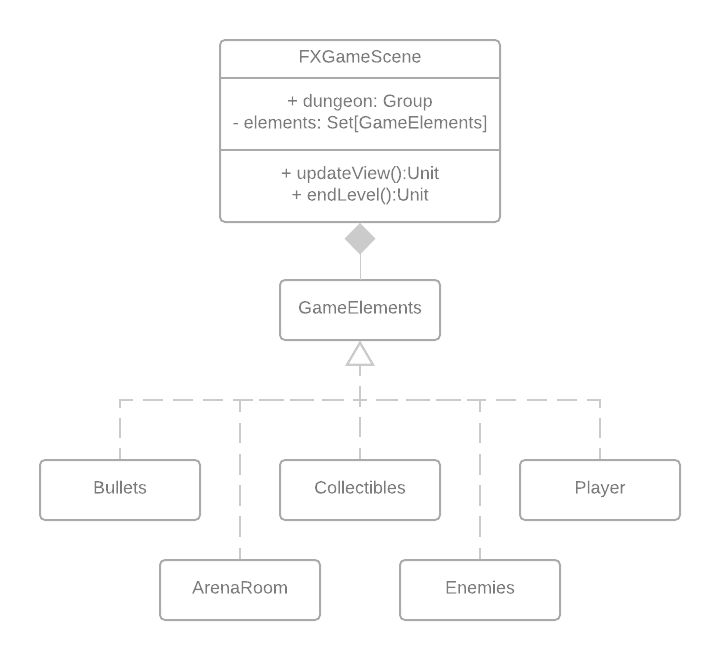
\includegraphics[width=15cm]{res/VIEW_Diagram.png}
  \caption{Organizzazione dell'arena di gioco}
  \label{view}
\end{figure}